% -------------------------------------------------------------------------
%  MusicFormats Library
%  Copyright (C) Jacques Menu 2016-2024

%  This Source Code Form is subject to the terms of the Mozilla Public
%  License, v. 2.0. If a copy of the MPL was not distributed with this
%  file, you can obtain one at http://mozilla.org/MPL/2.0/.

%  https://github.com/jacques-menu/musicformats
% -------------------------------------------------------------------------

% !TEX root = mfuserguide.tex

% -------------------------------------------------------------------------
\chapter{More examples}
% -------------------------------------------------------------------------


% -------------------------------------------------------------------------
\section{Jianpu output}
% -------------------------------------------------------------------------

\xmlToLy\ can be used to produce scores in the \jianpu\ format, in which the notes piches are numbers relative to the scale instead of graphic elements:
\begin{lstlisting}[language=Terminal]
jacquesmenu@macmini: ~/musicformats-git-dev/musicxmlfiles > xml2ly basic/Anacrusis.xml -output-file-name Anacrusis_Jianpu.ly -jianpu -title "Anacrusis score in Jianpu format"
\end{lstlisting}

This option needs lilypond-Jianpu to be accessible to LilyPond. This is available at \url{https://github.com/nybbs2003/lilypond-Jianpu/jianpu10a.ly}.

The key in this example is C major. The resulting \fileName{MinimalScore_Jianpu.ly} leads to:\\
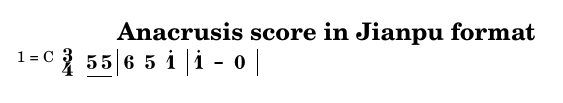
\includegraphics[scale=1]{../mfgraphics/mfgraphicsAnacrusis_Jianpu.png}

This is to be compared with:\\
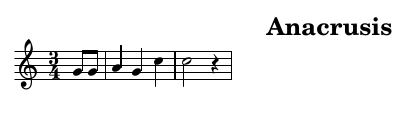
\includegraphics[scale=1]{../mfgraphics/mfgraphicsAnacrusis.png}


% -------------------------------------------------------------------------
\section{Braille output}
% -------------------------------------------------------------------------

The same score can also be produced in braille, with an interpretation of the 6-doc cells for debug in this case, by \xmlToBrl:
\begin{lstlisting}[language=Terminal]
jacquesmenu@macmini > xml2brl basic/Anacrusis.xml -auto-output-file-name -utf8d --use-encoding-in-file-name
\end{lstlisting}

This results in fileName{Anacrusis_UTF8Debug.brf}, which displays as:\\
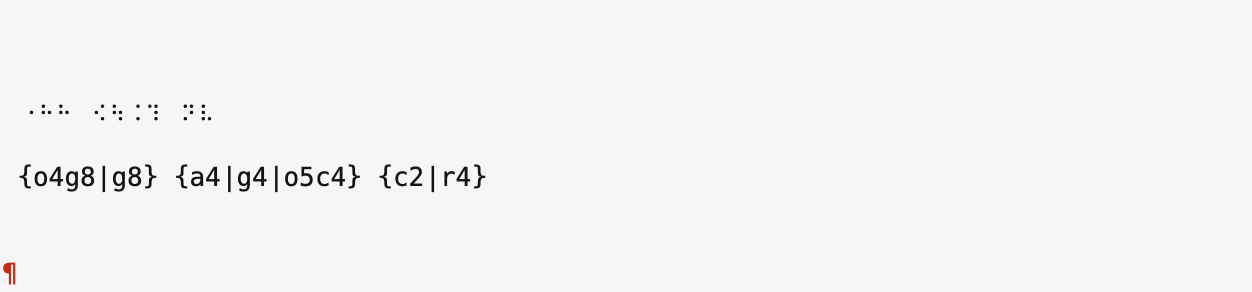
\includegraphics[scale=1]{../mfgraphics/mfgraphicsAnacrusis_Braille.png}

The \code{obj*} indicate the octave, and notes pitches and rests use \lily\ syntax.


% -------------------------------------------------------------------------
\section{Guido output}
% -------------------------------------------------------------------------

\guido\ is a textual representation of music scores. Converting \mxml\ to \guido\ is the reason why \fober\ created \libmusicxml\ in the first place.

\mf's \xmlToGmn\ is a \multiPass\ converter when \xmlToGuido\, a part of \libmusicxml, has two passes and only usea a \mxsrRepr\ representation.

\begin{lstlisting}[language=Terminal]
jacquesmenu@macmini: ~/musicformats-git-dev/musicxmlfiles > xml2gmn basic/Anacrusis.xml
{[ \staff<1> \set<autoHideTiedAccidentals="on"> \title<""> \auto<autoInstrPos="on"> \instr<"Voice"> \barFormat<style= "system", range="1"> \bar<hidden="true"> \key<0> \meter<"3/4", autoMeasuresNum="system"> \stemsUp \beamBegin:1 g/8 \stemsUp g/8 \beamEnd:1 \bar<hidden="true"> \stemsUp \beamsOff a/4 \stemsUp \beamsOff g/4 \stemsDown \beamsOff c2/4 \bar<hidden="true"> \stemsDown \beamsOff c/2 _/4 ]
  }
\end{lstlisting}

This can be viewed and edited on \fober 's \url{https://guidoeditor.grame.fr/#}:\\
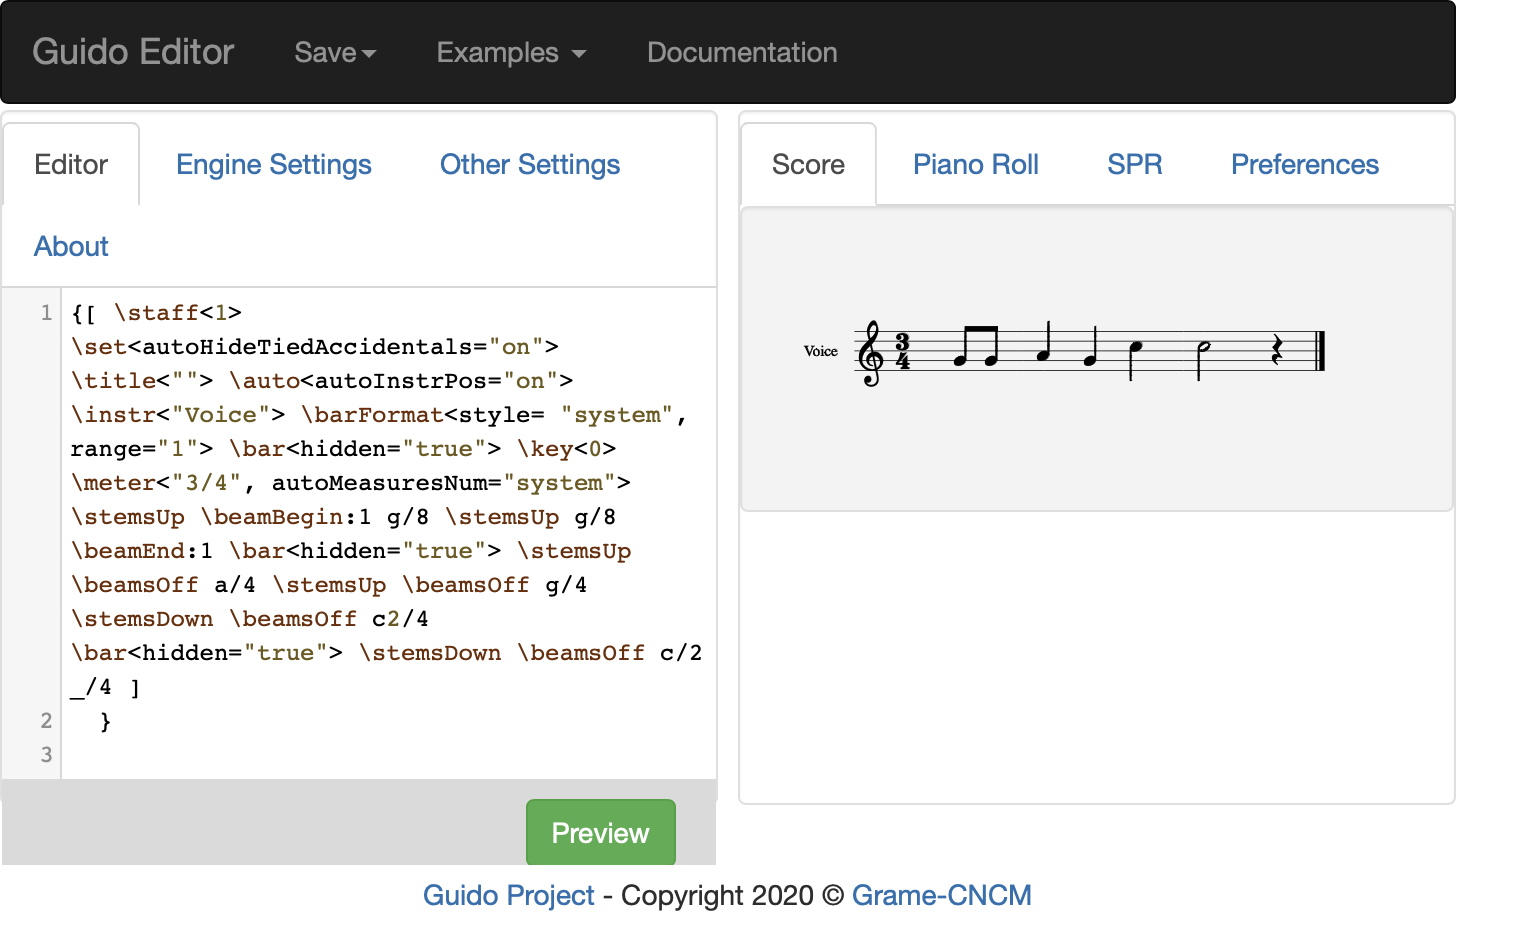
\includegraphics[scale=0.7]{../mfgraphics/mfgraphicsAnacrusis_Guido.png}


% -------------------------------------------------------------------------
\section{MusicXML output}
% -------------------------------------------------------------------------

\xmlToXml\ is meant for applying transformations to \mxml\ data. For example, \gitmxmlfile{basic/Anacrusis.xml} contains:
\begin{lstlisting}[language=Terminal]
jacquesmenu@macmini: ~/musicformats-git-dev/musicxmlfiles > cat basic/Anacrusis.xml
<?xml version="1.0" encoding="UTF-8"?>
<!DOCTYPE score-partwise PUBLIC "-//Recordare//DTD MusicXML 3.0 Partwise//EN" "http://www.musicxml.org/dtds/partwise.dtd">
<score-partwise>
  <work>
    <work-title>Anacrusis</work-title>
    </work>

	<!-- ... ... ... />

  </score-partwise>
\end{lstlisting}

We can obtain another \mxml\ file with this command, changing the work title, adding a work number and using an alto clef instead of a treble clef:
\begin{lstlisting}[language=Terminal]
jacquesmenu@macmini: ~/musicformats-git-dev/musicxmlfiles > xml2xml basic/Anacrusis.xml -output-file-name Anacrusis_From_xml2xml.xml -msr-replace-clef treble=alto -work-title "Anacrusis from xml2ml with alto clef" -work-number 317
\end{lstlisting}

The resulting file \fileName{Anacrusis_From_xml2xml.xml} contains:
\begin{lstlisting}[language=MusicXML]
jacquesmenu@macmini: ~/musicformats-git-dev/musicxmlfiles > cat Anacrusis_From_xml2xml.xml
<?xml version="1.0" encoding="UTF-8" standalone="no"?>
<!DOCTYPE score-partwise PUBLIC "-//Recordare//DTD MusicXML 3.1 Partwise//EN"
			"http://www.musicxml.org/dtds/partwise.dtd">
<score-partwise version="3.1">
    <!--
==================================================
Generated by xml2xml v0.9.5 (October 6, 2021)
on Monday 2022-02-14 @ 08:05:54 CET
from "basic/Anacrusis.xml"
==================================================
-->
    <work>
        <work-number>317</work-number>
        <work-title>Anacrusis from xml2ml with alto clef</work-title>
    </work>

	<!-- ... ... ... />

    <part id="P1">
        <measure number="0">
            <attributes>
                <divisions>2</divisions>
                <key>
                    <fifths>0</fifths>
                </key>
                <time>
                    <beats>3</beats>
                    <beat-type>4</beat-type>
                </time>
                <clef>
                    <sign>C</sign>
                    <line>3</line>
                </clef>
            </attributes>

	<!-- ... ... ... />

  </score-partwise>
\end{lstlisting}

Let's convert this to \lily\ with \xmlToLy\ into \fileName{Anacrusis_From_xml2xml.ly}:
\begin{lstlisting}[language=Terminal]
jacquesmenu@macmini: ~/musicformats-git-dev/musicxmlfiles > xml2ly Anacrusis_From_xml2xml.xml -auto-output-file-name
\end{lstlisting}

The resulting score is:\\
\includegraphics[scale=0.7]{../mfgraphics/mfgraphicsAnacrusis_From_xml2xml.png}

